\chapter{从磁岛图像到实验检验：实验究竟测到了什么}
\label{tm:chap:experiments}

\section{先把三个不同的问题分开}

理论推导得到的是一个本征模：给定平衡、边界条件和闭合，求扰动的空间结构及增长率。实验仪器直接给出的却可能是线圈电压、辐射强度或粒子照相。要把两者连起来，需要经过诊断标定、几何重建和模型比较。以下三个命题的证据强度不同。

\begin{enumerate}
  \item \textbf{存在磁岛。}需要看到闭合的扰动磁通面、O 点与 X 点，或多个相互支持的间接信号。这回答拓扑问题。
  \item \textbf{磁岛由某种撕裂不稳定性产生。}还要识别自由能、背景演化、种子扰动和可能的外部强迫。已有磁岛也可能是外部扰动驱动的。
  \item \textbf{某个具体增长率公式被检验。}应测量平衡、波数、耗散、线性区间的扰动幅度以及不确定度，然后比较公式。看到一串岛，尚不等于测得了 FKR 的 $S_a^{-3/5}$ 标度。
\end{enumerate}

特别要区分\emph{随时间增大}和\emph{线性本征模的指数增长}。若电流片在观察期间持续变薄，$a(t)$、$\Delta'(t)$、$S_a(t)$ 同时改变，用一条固定平衡的 $e^{\gamma t}$ 拟合就可能失去意义。若岛已进入 Rutherford 阶段，$W$ 可以近似随时间线性变化，但这不是“线性扰动理论阶段”：前一个“线性”描述曲线形状，后一个“线性”描述方程对扰动幅度的截断。

本章选择三类原始实验：托卡马克中的新经典撕裂模控制、专门重联装置中的碰撞性双流体电流片，以及激光产生的快速演化高 $\beta$ 电流片。它们检验理论的不同部分，不能排成一条由低到高的“模型正确率”。文中重新绘制的图全部为教学示意或解析曲线，\textbf{没有把自设数据画成实验结果}。原论文的图号用于指导读者回到原始证据。

\section{从平板共振面走向托卡马克有理面}

\subsection{为什么会出现 \texorpdfstring{$q=m/n$}{q=m/n}}

在大环径、近圆截面的近似下，以 $r$ 表示小半径，$R$ 表示大半径，$\theta$ 为极向角，$\zeta$ 为环向角。设一个螺旋扰动的相位为
\begin{equation}
 \alpha=m\theta-n\zeta-\omega t,
 \qquad m,n\in\mathbb Z.
 \label{tm:helical_phase}
\end{equation}
整数性来自角度增加 $2\pi$ 后物理量必须单值。在圆柱近似下，
\begin{equation}
 \B\cdot\nabla\alpha
 =\frac{mB_\theta}{r}-\frac{nB_\zeta}{R}.
\end{equation}
定义安全因子
\begin{equation}
 q(r)\simeq\frac{rB_\zeta}{RB_\theta},
 \qquad
 k_\parallel\equiv\frac{\B\cdot\nabla\alpha}{B}
 =\frac{B_\zeta}{RB}\left(\frac{m}{q}-n\right).
 \label{tm:q_resonance}
\end{equation}
当 $q(r_s)=m/n$ 时，$k_\parallel(r_s)=0$。这表示沿平衡磁力线走动时，该扰动的螺旋相位在共振面上不变。它是前面平板模型 $\vct{k}\cdot\B_0=0$ 的环形对应物。\emph{并不是磁场本身变成零}：托卡马克通常有很强的环向磁场。对真实成形平衡，$q$ 通过磁力线的一周积分定义，仍有有理面共振；上述简单局地表达式只用于建立直观。

写 $x=r-r_s$，在 $|x|$ 足够小时作泰勒展开，
\begin{equation}
 k_\parallel(x)\simeq k_\parallel'(r_s)x,
 \qquad
 k_\parallel'(r_s)=-\frac{B_\zeta}{RB}\frac{m q'(r_s)}{q_s^2}.
 \label{tm:kpar_shear}
\end{equation}
因为括号 $m/q-n$ 在 $r_s$ 恰好为零，对前因子求导所得的项消失。$q'$ 所表达的磁剪切，正是局地 $B_y\simeq B'x$ 中 $B'$ 的对应物。

\begin{figure}[htbp]
 \centering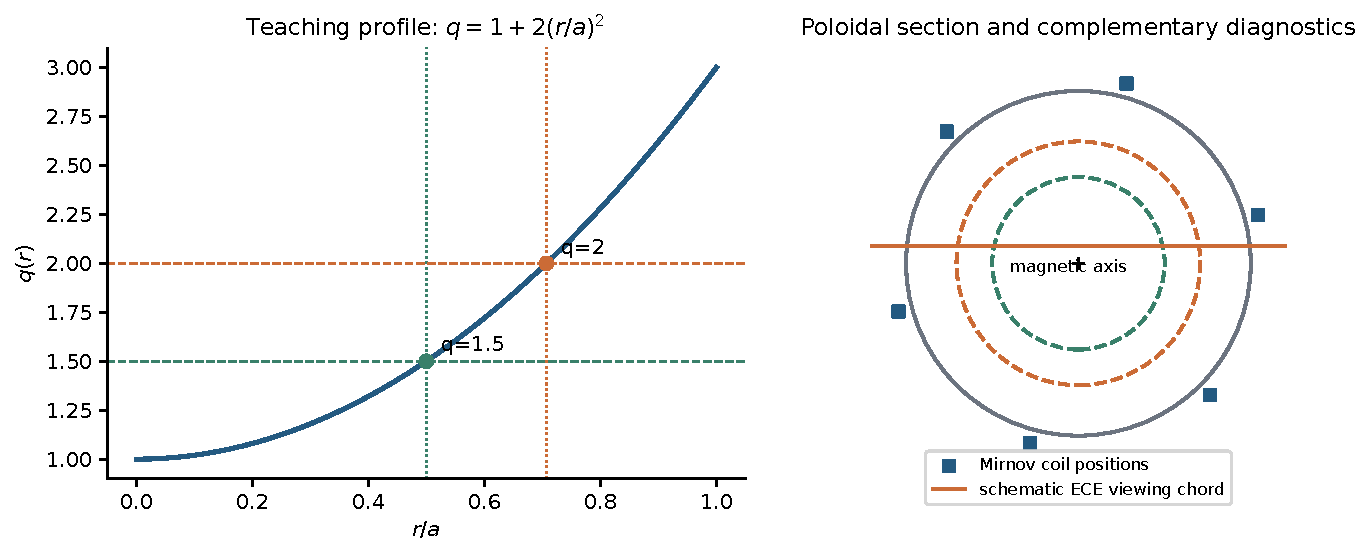
\includegraphics[width=0.94\textwidth]{figures/tm_rational_diagnostics.pdf}
 \caption{自设的托卡马克教学几何。左：$q=1+2(r/a)^2$ 的 $q=3/2$ 与 $q=2$ 有理面。右：圆截面磁面、外部 Mirnov 线圈与一条 ECE 观测弦的示意。此图不对应 DIII-D 的实际成形平衡，也没有模拟辐射传输。}
 \label{tm:fig:rational}
\end{figure}

\subsection{“一个 \texorpdfstring{$m/n=2/1$}{m/n=2/1} 模”意味着什么}

固定 $\zeta$，相位随 $\theta$ 变化两周；固定 $\theta$，随 $\zeta$ 变化一周。这并不意味着任何一张相机照片都必然显示两个清晰孤立的圆斑。视线积分、岛的相位、磁面形状和诊断响应会改变图像。实际模式识别通常同时使用多个线圈的相位、平衡重建的 $q$ 剖面以及内部温度扰动。

\section{从仪器信号重建岛：一步一步解释}

\subsection{Mirnov 线圈首先测到的是电压}

小线圈包围面积 $A$，匝数 $N$，若磁场在其面积内近似均匀，法拉第定律给出
\begin{equation}
 V(t)=-N A_{\rm eff}\frac{\dd\delta B_{\perp}}{\dd t}.
 \label{tm:mirnov_voltage}
\end{equation}
这里 $\perp$ 是线圈法向，而非必然等于平衡场的垂直方向；有效面积还取决于方向和标定。测得电压后，通过传递函数校正和时间积分才得到磁扰动。积分常数、低频漂移、导体壁屏蔽及线缆相位都应处理。

若单一模式近似为
\begin{equation}
 \delta B_j(t)=A(t)\cos\!\left(m\theta_j-n\zeta_j-\omega t+\alpha_0\right),
 \label{tm:mirnov_B}
\end{equation}
同一时刻两个探头的相位差满足
\begin{equation}
 \Delta\alpha=m\Delta\theta-n\Delta\zeta\pmod {2\pi}.
 \label{tm:phase_difference}
\end{equation}
知道探头位置后，拟合整数 $m,n$。只有一个极向阵列无法独立确定环向模数；稀疏阵列还会产生相位混叠。实际需要多个位置、频带相干性和连续相位展开，而不是用两点决定所有模式。

\begin{figure}[htbp]
 \centering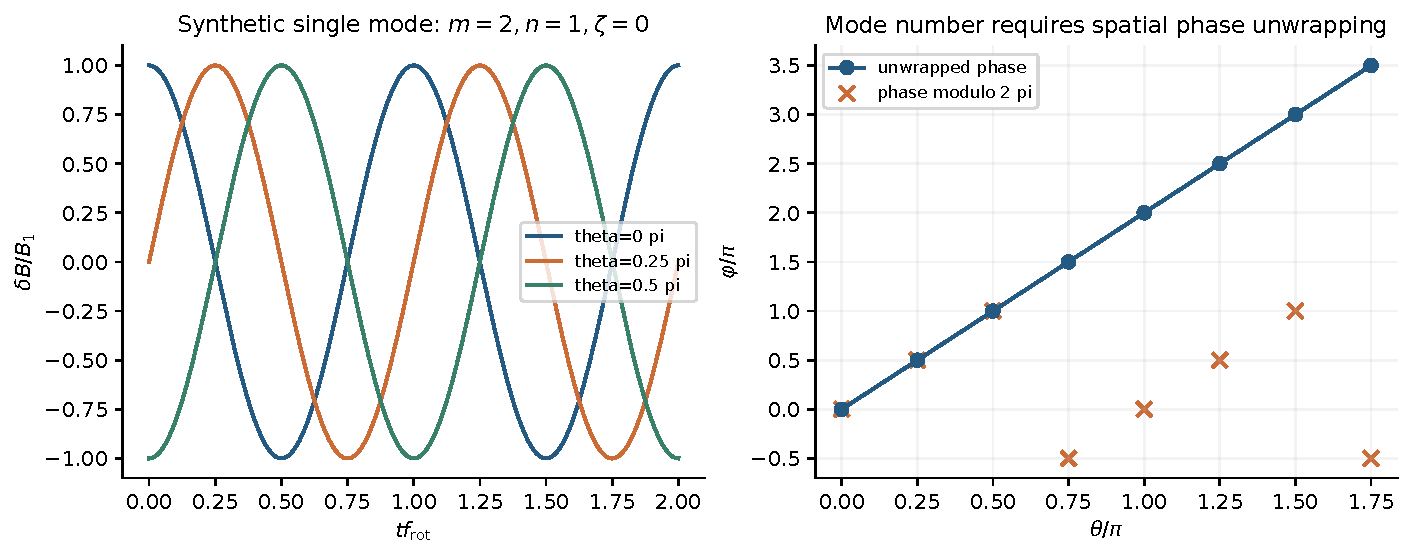
\includegraphics[width=0.94\textwidth]{figures/tm_mirnov_phase.pdf}
 \caption{合成的 $m=2,n=1$ 磁场信号。左图三个极向位置的时间相位不同；右图展示相位的 $2\pi$ 包裹与展开。画的是已还原的 $\delta B$，不是原始线圈电压；没有噪声、壁响应或多模叠加，不是实验数据。}
 \label{tm:fig:mirnov}
\end{figure}

对 $A(t)=A_0e^{\gamma t}$ 求导，电压含有两个分量：
\begin{equation}
 V=-NA_{\rm eff}A(t)\,[\gamma\cos\alpha+\omega\sin\alpha].
\end{equation}
电压包络为 $NA_{\rm eff}A\sqrt{\gamma^2+\omega^2}$。当 $|\omega|\gg\gamma$，电压幅度主要正比于 $|\omega|A$。因此模式旋转减慢时，电压可降低而磁扰动并未同比降低；完全锁定且不再增长的岛甚至不产生持续感应电压。要宣称“岛消失”，不能只看到某个交流频带信号变小，还应结合低频/静态磁测量、温度结构或其他诊断。

\subsection{为什么磁岛会使温度变平}

沿磁场的电子热传导通常远强于跨场热传导。一个最简输运模型是
\begin{equation}
 \frac{\partial T_e}{\partial t}
 =\chi_\parallel\nabla_\parallel^2T_e+
   \chi_\perp\nabla_\perp^2T_e+Q_T,
 \label{tm:anisotropic_heat}
\end{equation}
其中 $\chi$ 为热扩散率（$\mathrm{m^2\,s^{-1}}$），$Q_T$ 是换算成温度变化率的源项。这是教学闭合，实际热通量还可能非局地且包含湍流。

磁岛形成后，一条闭合的螺旋磁力线访问原本不同半径的位置。沿线传热把这些位置的温差拉小，岛内温度便倾向于在螺旋磁通面上近似相等。穿过 O 点的径向剖面最容易出现平坦区；穿过 X 点或分离界附近则不同。岛旋转经过固定探头时，这种空间结构变成周期信号，跨越共振面的若干温度扰动通道还可能出现相位反转。

“出现岛就立即完全平坦”也不准确。扩散时间分别约为 $\tau_\parallel\sim L_\parallel^2/\chi_\parallel$ 和 $\tau_\perp\sim W^2/\chi_\perp$。小岛附近有效平行连接长度大，平行均温可能赶不上跨场补给及源项，形成有限宽度阈值。故没有显著温度平坦区，并不单独排除很小的磁岛；平坦区的宽度也不能未经诊断卷积就直接当成 $W$。

\subsection{ECE、软 X 射线和平衡重建各补哪一块信息}

电子回旋辐射（ECE）的观测频率与局地磁场有关：在最简非相对论近似下，
\begin{equation}
 f\simeq s f_{ce}=s\frac{eB}{2\pi m_e},\qquad s=1,2,\ldots .
\end{equation}
若等离子体在该频带光学厚、电子接近热分布，并正确处理传播与相对论展宽，亮温可以用来推断电子温度。由于 $B$ 随位置变化，多频通道近似对应不同径向位置，从而看到岛导致的温度结构。频率通道的有限宽度意味着有限空间分辨率；非热电子、光学薄区域或反射会破坏简单的“亮温等于 $T_e$”。

软 X 射线（SXR）的单条观测弦更接近
\begin{equation}
 I_{\rm SXR}\propto\int_{\rm chord} n_e^2\,Lambda(T_e,Z_{\rm eff},\ldots)\,\dd l,
\end{equation}
其中 $\Lambda$ 包括辐射过程、杂质和探测器谱响应。它是视线积分，并非单点温度计。多弦层析及相位分析能识别旋转结构，但密度、温度与杂质变化可能互相混淆。磁测量给模数，ECE/SXR 给内部结构，动理学剖面和平衡重建给有理面位置，组合证据更有说服力。运动斯塔克效应（MSE）可提供磁场方向约束，帮助平衡重建推断 $q(r)$；$q$ 并非由一支 Mirnov 线圈直接读出。

\section{经典、NTM、强迫重联和锯齿：相似图像不等于相同驱动}

\subsection{新经典撕裂模的正反馈}

在环形装置中，粒子会受到磁场强度沿磁力线变化的影响；一部分粒子被磁镜俘获。碰撞、俘获与通过粒子的输运耦合，使压力梯度能够驱动自举电流（bootstrap current）。这里的“新经典”指把环形几何及俘获粒子纳入碰撞输运理论，不是“新提出的经典撕裂模”。自举电流的系数需要更完整的新经典输运计算，不能从平板不可压缩 MHD 自动推出。

对常见的托卡马克参数，岛内压力平坦化会降低本来由压力梯度维持的局地自举电流。这个缺额具有与岛同相的螺旋结构，进一步加强岛。这就形成
\begin{equation}
 \text{有限种子岛}\ \longrightarrow\ \text{压力平坦化}
 \ \longrightarrow\ \text{自举电流缺额}
 \ \longrightarrow\ \text{岛继续增大}.
\end{equation}
即使经典项 $\Delta'_{\rm class}<0$，附加驱动也可能使有限岛增长。小岛时的有限平坦化、极化电流和其他效应决定是否有阈值；因此 NTM 的有限幅度触发，与经典 FKR 从任意小扰动出发的线性不稳定性不是同一个问题。

\begin{figure}[htbp]
 \centering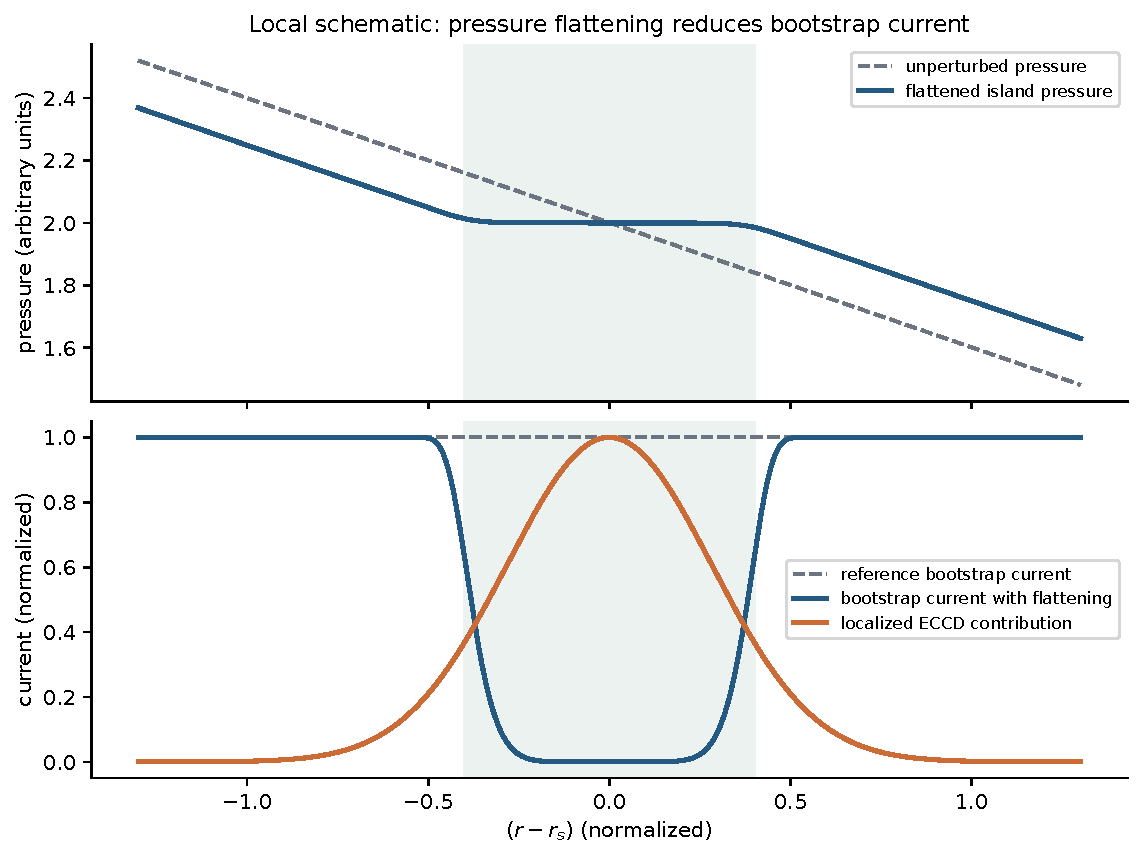
\includegraphics[width=0.94\textwidth]{figures/tm_bootstrap.pdf}
 \caption{自设的 NTM 教学图：压力平坦化、相应的自举电流缺额，以及在同一位置补充的局地 ECCD。曲线由脚本给定解析轮廓，仅解释反馈方向；不是 DIII-D 数据，也不是新经典输运方程的数值解。实际电流和驱动还依赖螺旋相位、岛宽、沉积宽度与偏心量。}
 \label{tm:fig:bootstrap}
\end{figure}

为保持量纲清楚，可把\emph{修正 Rutherford 方程的组织形式}写为
\begin{equation}
 \frac{I_1}{D_\eta}\frac{\dd W}{\dd t}
 =\Delta'_{\rm class}
 +\Delta'_{\rm BS}(W)
 +\Delta'_{\rm pol}(W)
 +\Delta'_{\rm CD}(W,\Delta r,w_{\rm CD})+\cdots .
 \label{tm:mre_structure}
\end{equation}
这里各个有效 $\Delta'$ 的单位都是 $\mathrm{m^{-1}}$；$\Delta r$ 为电流驱动相对有理面的偏心量，$w_{\rm CD}$ 为驱动分布宽度。$I_1\simeq0.823$ 对应前文特定全宽、局地电阻模型的归一化；真实环形模型经常吸收系数并使用不同长度。式\eqref{tm:mre_structure}是分类表达，\emph{不是给所有装置通用的精确闭合公式}。自举、极化、有限输运和电流驱动项的系数与符号应从所选模型求得，不能把平板系数与另一篇论文的宽度定义混用。

电子回旋电流驱动（ECCD）利用波对电子速度分布的非对称作用来驱动电流。若在岛的合适位置补回缺失电流，可产生稳定作用。它既需要足够总功率，也需要合适位置和窄的沉积轮廓：同样的总电流均摊到太宽区域，有效螺旋电流分量就小。

\subsection{其他几种容易混淆的情形}

\begin{itemize}
 \item \textbf{强迫重联：}外部共振磁场或边界运动提供扰动。一个经典线性稳定、$\Delta'<0$ 的平衡也可能形成有限磁岛；研究的是响应、穿透与重联过程，不能仅凭岛存在宣布自发线性不稳定。
 \item \textbf{锯齿：}托卡马克核心温度周期性缓慢上升、快速崩塌，常涉及 $q\simeq1$ 附近的 $m=n=1$ 内扭曲及重联。它包含重联物理，却不等于本讲义的静态 Harris 平板 FKR 问题；锯齿还可为别的有理面上的 NTM 提供种子。
 \item \textbf{磁岛链/plasmoid：}这是结构名称。可能来自电阻性撕裂、Hall/电子尺度撕裂、随时间变薄电流片的多模过程或其他动力学。需要尺度排序和演化证据识别具体机制。
\end{itemize}

\section{实验一：DIII-D 对 NTM 的定点电流驱动控制}
\label{tm:sec:diiid}

本节采用可完整取得的 \citet{TMPetty2003} 原始技术报告 GA--A24317，版本为 2003 年射频会议预印本。PDF 共 7 页，其中正文为报告页 1--4。\textbf{它不是对随后正式期刊版本的逐页核读替代品。}图 1 给出成形平衡、回旋共振面、波轨迹、ECE 与 MSE 几何；图 2--4 分别提供控制时间轨迹、位置扫描和模型比较。

\paragraph{装置、驱动和测量。}
DIII-D 中的 $m/n=2/1$ NTM 位于 $q=2$ 面。实验使用最高合计 $2.7\,\mathrm{MW}$ 的吸收 ECCD 功率，回旋管频率 $110\,\mathrm{GHz}$。文中的约 $40\,\mathrm{kA}$ 驱动电流是 CQL3D 计算结果，不是独立的直接电流探针测量。外部 Mirnov 信号跟踪 $n=1$ 磁扰动；$q=2$ 位置来自平衡重建，ECCD 位置来自射线追踪。

\paragraph{关键比较。}
原文图 2 对比完全和部分抑制的放电；图 3 扫描环向磁场，使 ECCD 沉积经过共振位置，磁扰动在两者对齐附近最小。完全抑制案例的反馈调整约为 $0.01\,\mathrm T$，相当于中平面沉积位置移动约 $0.9\,\mathrm{cm}$。这说明“放进功率”之外，\emph{把电流驱动放在正确位置}是关键变量。

\paragraph{模型比较到什么程度。}
图 4 用修正 Rutherford 模型比较\emph{部分抑制扫描}中最小岛宽：测得约 $8\,\mathrm{cm}$，由沉积全半高宽约 $3.3\,\mathrm{cm}$ 的模型匹配；射线追踪给出的宽度为 $2.6\,\mathrm{cm}$，允许的比较范围约 $2.6$--$3.9\,\mathrm{cm}$。不要把这里的 $8\,\mathrm{cm}$ 误写成完全抑制案例的初始岛宽。图中理论误差条包含回旋管功率的 $10\%$ 不确定性。

\paragraph{可以得出与不能得出的结论。}
该实验直接支持局地电流驱动能够控制 NTM，以及控制对共振位置的敏感性。它不是经典 FKR 线性增长率的检验；$q$ 位置、沉积轮廓和驱动电流包含反演或模型。用岛宽约束沉积宽度时，参数是经模型推断的，不应又把同一个岛宽当作完全独立的预测成功。放电还通过中性束反馈调节能量和 $\beta$，评估控制效果要同时看这些轨迹。上述结论均对应原文图 1--4 及其说明。\citep{TMPetty2003}

\section{实验二：MRX 的碰撞性双流体电流片和岛链}
\label{tm:sec:mrx}

\citet{TMJaraAlmonte2016} 在磁重联实验装置 MRX 的氩等离子体中观测到岛链。所读作者稿共 5 页，对应 PRL 117, 095001。它特别适合纠正“Hall 效应出现就一定无碰撞”的误解。

\paragraph{参数与尺度。}
上游典型 $n_e\simeq5\times10^{19}\,\mathrm{m^{-3}}$、$T_e\simeq3\,\mathrm{eV}$，片内约 $2\times10^{20}\,\mathrm{m^{-3}}$、$4\,\mathrm{eV}$。原文代表性排序为
\begin{equation}
 d_e\sim0.5\,\mathrm{mm}
 <\lambda_{\rm mfp}\sim2\,\mathrm{mm}
 <\delta\sim9\,\mathrm{mm}
 \ll d_i\sim200\,\mathrm{mm},
 \label{tm:mrx_scales}
\end{equation}
其中 $\delta$ 是电流片半厚度。离子不能在片尺度上简单地与电子共同运动，但片厚又比电子惯性尺度和电子平均自由程大；因此 Hall 物理与碰撞性电阻可以同时重要。

\paragraph{怎样认出岛。}
约 400 个拾取线圈测量三分量磁场，最好采样间距跨片约 $6\,\mathrm{mm}$、沿片约 $3\,\mathrm{cm}$。原文图 2 展示重建磁通轮廓和法向磁场翻转；作者还用局部磁矢量的绕数识别 O/X 点，检查插值是否凭空产生小岛。原文坐标与本讲义不同：其径向跨片方向对应本讲义 $x$，出流方向对应 $y$，出平面电流方向对应 $z$，不能照搬下标。

\paragraph{统计结果与模型解释。}
图 3 比较平均岛数、长宽比与 Lundquist 数；研究包含约 200 次放电和 500 次形成事件。许多岛出现在 $S<100$ 的范围。图 4--5 将岛形成与重联率变化联系起来，超过四分之三事件的重联率增加，平均一个岛的形成对应约 $10\%$ 的归一化率增加；原文对率给出约 $10\%$ 的保守不确定性。这是事件统计，不表示每个岛都会精确产生同样增益。\citep{TMJaraAlmonte2016}

\paragraph{为何不能直接拿经典临界数判错。}
常被引用的 $S\sim10^4$ 是特定高 $S$ 电阻 MHD 电流片及其形成条件下的参考，不是“所有岛的普适门槛”。MRX 的 Hall 尺度、可压缩性、有限长宽比和持续驱动都影响稳定性。原文将结果解释为电阻性电子撕裂，同时明确指出，含实际密度、Hall 场和几何的二维线性比较仍不充分。$6\,\mathrm{mm}$ 的探头间距不能分辨 $0.5\,\mathrm{mm}$ 电子惯性层；观测到拓扑与 Hall 场，也不能单独给出所有电子解冻项的精确预算。图 3 的总体散布与均值误差是不同误差条，读图时亦应区分。\citep{TMJaraAlmonte2016}

\section{实验三：激光高 \texorpdfstring{$\beta$}{beta} 等离子体中的 plasmoid 证据}
\label{tm:sec:laser}

\citet{TMPearcy2024} 使用 OMEGA EP 激光驱动两个磁化等离子体泡碰撞。所读为作者机构公开的 PRL 132, 035101，7 页，包括方法附录；它把磁场照相、反演及有限时间分辨率的问题展示得很清楚。

\paragraph{如何产生和拍摄电流片。}
两个 $930\,\mathrm J$、$1\,\mathrm{ns}$ 的相互作用激光脉冲照射 CH 薄膜，产生膨胀磁化泡。质子照相利用质子穿过磁场时的偏转，把偏转映射为探测面上的通量明暗。不同能量的质子具有不同飞行时间，从同次实验得到多个时间切片。图 1 给出装置；图 2--3 比较质子图像与重建的磁场、磁通和电流；图 4 检查法向场的符号变化。

\paragraph{实测与反演量要分开。}
直接记录的是质子在胶片上的空间分布。路径积分磁场由反问题求得，再推断磁通岛和电流结构；局地 $B$ 还需要场区路径长度假设。文中典型 $B\sim40$--$70\,\mathrm T$、$\beta\sim10$，表 I 给出 $L\sim2000\,\mu\mathrm m$、电流片宽度 $20$--$60\,\mu\mathrm m$、$d_i\sim55\,\mu\mathrm m$、$d_e\sim1\,\mu\mathrm m$。这里实验电流宽度按电流轮廓全半高宽定义，不能当成前文 Harris 参数 $a$。

\paragraph{观察到了什么。}
重建磁通出现约 $100$--$200\,\mu\mathrm m$ 的岛结构；图 4 的场翻转提供进一步检验。图 5 的电流轮廓显示片宽变化；图 6 跟踪岛宽。中央和右侧岛在误差内没有可辨认增长；左侧结构的快速变宽受边缘流动和几何影响，作者没有把它直接当作线性撕裂增长率。\citep{TMPearcy2024}

\paragraph{限制决定了应如何解释。}
这是一张快速形成且持续受驱动的电流片，未必满足静态 Sweet--Parker 或 FKR 假设。反演涉及入射质子通量、轨迹映射、能量展宽和磁偏转主导的假设；测得的是沿视线积分量，没有同时的侧向三维重建。部分等离子体参数来自名义相同驱动条件下的另一组 Thomson 散射实验，并非所有量都在同一次照相放电里同时测得。它支持高 $\beta$ 重联中存在 plasmoid 及离子尺度附近的片结构，但不构成对某一普适 $\gamma(S)$ 的直接测量。下一章会算出：在其可用时间窗里，典型重联速度预期造成的岛宽变化完全可能低于空间分辨率。\citep{TMPearcy2024}

\section{把三个实验放回理论学习路线}

\begin{table}[htbp]
\centering\small
\begin{tabular}{p{0.16\textwidth}p{0.35\textwidth}p{0.36\textwidth}}
\toprule
研究 & 最直接支持的物理 & 没有由此自动完成的检验\\
\midrule
DIII-D NTM & 局地电流驱动及对齐可抑制有限岛；修正 Rutherford 模型有可检验的控制含义 & 经典 FKR 线性指数和完整新经典闭合的独立验证\\[3pt]
MRX 岛链 & 碰撞性电阻与双流体尺度可共存；磁拓扑与重联率有统计联系 & 实际二维平衡的完整本征值问题、每个电子解冻项和三维效应\\[3pt]
OMEGA EP & 快速演化高 $\beta$ 电流片中磁岛的成像证据 & 在分辨率不足的短窗内准确测得线性增长率；排除所有三维结构\\
\bottomrule
\end{tabular}
\caption{按原始论文证据范围作出的教学比较。各行的限制不否定实验结果，而是说明结果实际约束了理论的哪一部分。}
\label{tm:tab:experiments}
\end{table}

以后阅读一篇撕裂模实验论文，可以依次检查：扰动究竟是自发还是外加；模数及共振面如何确定；幅度是磁通、磁场、岛宽还是线圈电压；背景是否近似静态；岛宽定义和时间区间是否与理论一致；测量误差能否区分候选模型。这样才能从“图像很像”推进到“某个定量理论受到约束”。本讲义的源文件同时保存原文版本、阅读范围和图号，便于逐项回查，而没有将候选下载量改写成全库全文核读数量。
